\documentclass[10pt,a4paper]{article}

\usepackage[a4paper, left=2.5cm, right=2cm, top=2.5cm, bottom=2cm]{geometry}
\usepackage{newtxtext,newtxmath}
\usepackage{tabularx}
\usepackage{amsmath}
\usepackage{algorithmic}
\usepackage{graphicx}
\usepackage{textcomp}
\usepackage{xcolor, dcolumn}
\usepackage{pgfplots}
\pgfplotsset{compat=1.9}
\usepackage{tikz}
\usepackage{gensymb}
\usepackage{caption}
\usepackage{enumitem}
\usepackage{titlesec}
\usepackage{fancyhdr}
\usepackage{indentfirst}
\usepackage{setspace}
\usepackage[hyphens]{url}

\captionsetup{font={small,bf}, labelfont=bf, skip=6pt}
\captionsetup[table]{position=above, skip=6pt}

\titleformat{\section}{\normalfont\fontsize{12}{14}\bfseries}{\thesection}{1em}{}
\titleformat{\subsection}{\normalfont\fontsize{12}{14}\bfseries}{\thesubsection}{1em}{}
\titleformat{\subsubsection}{\normalfont\fontsize{10}{12}\bfseries\itshape}{\thesubsubsection}{1em}{}

\titlespacing{\section}{0pt}{12pt}{6pt}
\titlespacing{\subsection}{0pt}{12pt}{6pt}
\titlespacing{\subsubsection}{0pt}{12pt}{3pt}

\setlength{\parskip}{3pt}
\setlength{\parindent}{1em}
\onehalfspacing

\usepackage[numbers,sort&compress]{natbib}

\begin{document}

\begin{center}
    {\fontsize{14}{17}\bfseries Corn Diseases Classification Using Grey-Level Co-Occurrence Matrix and Random Forest Algorithm\par}
    \vspace{12pt}
    {\large
        Firmansyah Sundana\textsuperscript{1}, Fitri Utaminingrum\textsuperscript{2}\\
    }
    \vspace{6pt}
    \small
    \textsuperscript{1}Graduate Program Of Computer Science, Faculty of Computer Science, Brawijaya University, Malang, Indonesia\\
    \textsuperscript{2}Computer Vision Research Group, Faculty of Computer Science, Brawijaya University, Malang, Indonesia\\
    \vspace{3pt}
    \{sundana, f3\_ningrum\}@ub.ac.id\\
    \vspace{6pt}
    Received xx month xxxx; accepted xx month xxxx
\end{center}

\vspace{6pt}
\begin{center}
    \textbf{\fontsize{10}{12}\selectfont Abstract}
\end{center}
\noindent Corn diseases are a primary concern in agriculture, leading to significant crop failure and economic losses for businesses reliant on corn supplies. Effective disease prevention before harvest is essential, yet existing classification methods often need to be revised, complicating disease management efforts. This study presents an advanced approach to improve the accuracy of corn disease classification by leveraging computer vision technology. The method begins with the U-Net segmentation model, which precisely isolates corn leaves from their background, facilitating the extraction of crucial plant features. These features are then analyzed using the Gray-Level Co-occurrence Matrix (GLCM) technique to capture essential texture information. To further enhance classification accuracy, Principal Component Analysis (PCA) is applied to select the most relevant features, reducing dimensionality and improving model efficiency. The Random Forest algorithm then classifies the extracted features into disease categories. The proposed method achieved an accuracy rate of up to 87\% and low time computation, indicating its effectiveness in accurately identifying corn leaf diseases. These results underscore the potential of this approach to significantly reduce the economic impact of corn diseases by enabling more reliable and timely disease detection.

\vspace{6pt}
\noindent\textbf{Keywords:} GLCM, image classification, computer vision, corn disease, random forest

\section{Introduction}

In 2023, the corn harvest area in Indonesia reached 2.49 million hectares \cite{bps}, highlighting the importance of corn as a vital commodity due to the high demand in various industrial sectors. However, the large area of corn production is a factor in corn's vulnerability to pathogen attacks. Pathogen attacks potentially reduce crop yields, leading to economic losses to a certain extent.

The agricultural sector has embraced innovative technologies like machine learning and IoT, leading to the emergence of precision agriculture \cite{Dhanaraju2022, Rehman2022}. This method utilizes IoT devices and sensors for identifying and categorizing items in farmland, including vegetation, soil, and the environmental conditions of the land. Previous studies have leveraged this development by developing reliable classification algorithms for various tasks, including the classification of plant diseases \cite{Ramesh2018,Sajitha2024}.

This classification problem invites various research in artificial intelligence to develop methods and models to distinguish diseases on plant leaves accurately. Research conducted by Sajitha et al. \cite{Sajitha2024} compiles various current approaches that try to solve the problem of disease detection and classification in plants. This research separates traditional machine learning methods from deep learning, which is applied to classify and detect plant diseases. However, few studies have focused on corn \cite{Pardede2018,Aurangzeb2020}. In addition, the performance of traditional machine learning models is entirely accurate \cite{Harakannanavar2022, Wang2020}, but still less accurate than deep learning models based on convolutional neural networks (CNN) \cite{Shoaib2022, Kabir2021, Pandian2022}.

Applying machine learning and deep learning has become the central axis in various types of image research \cite{Demilie2024,Ashwini2024,hatice}. While deep learning has obtained satisfactory accuracy results in classifying plant diseases, it requires extensive resources to be applied and requires more computation time than traditional machine learning \cite{Utaminingrum2023}. Research conducted by \cite{Jadhav2021,Durairaj2020,Hossain2019} applied a gray-level co-occurrence matrix (GLCM) to extract image texture features by applying statistical analysis to neighboring pixels. The results of GLCM texture extraction can show the differences in corn leaf diseases in detail. However, segmentation is needed to distinguish leaves from their background to get adequate marks. Therefore, our proposed method offers a more practical and accessible solution by combining CNN-based image processing methods with a traditional machine learning model. This hybrid technique easily applies to classification problems that rely on IoT or mobile devices. It is a viable option for most farmers, including those in Indonesia, who often only have smartphones with moderate computing capabilities \cite{David2023}.

This study offers a hybrid method, the UNet-GLCM-Random Forest, where UNet is the state-of-the-art image segmentation. UNet, a convolutional neural network, is combined with more traditional extraction and classification methods to reduce the high computing needs.

Our proposed method offers a more practical and accessible solution by combining CNN-based image processing methods with a traditional machine learning model. This hybrid technique easily applies to classification problems that rely on IoT or mobile devices. It is a viable option for most farmers, including those in Indonesia, who often only have instruments with moderate computing capabilities. It also can significantly maintain the appropriate accuracy and availability of tools used in precision agriculture to classify diseases in corn without constraint in computing resources \cite{Nawrocki2023} and time complexity \cite{Theodoropoulos2023}. This method could be a game-changer for the agricultural sector, offering a promising solution to the persistent challenge of disease outbreaks in corn.

\section{Method}

\subsection{Proposed Method}

This research applies a model based on computer vision and machine learning. We propose the U-Net+GLCM+Random Forest method to classify corn diseases by referring to the symptoms on the leaves. The model's overall structure can be seen in the Fig. \ref{fig:proposedmethod}. The corn samples used were Healthy and Non-Healthy, with three classes of Non-Healthy, including common rust, northern leaf blight, and gray leaf spot. The image size used is $256 \times 256$ pixels. Before segmenting the image, Roboflow annotates it to separate the background from the leaves. The annotation results train the U-Net model for segmentation. Feature extraction in segmented images applies the Gray-Level Co-Occurrence Matrix technique.The extracted features are then selected using the Principal Component Analysis method to reduce the dimensionality of the training data and prevent overfitting. 

% The Random Forest classifier was chosen for its robustness in handling high-dimensional data and its ability to generalize well with relatively small datasets. Compared to deep learning methods like CNNs, Random Forest requires less computational power, making it suitable for mobile and IoT devices with limited resources. While deep learning models such as CNNs often achieve high accuracy, they require large datasets and computational resources, which may not be practical for real-time field use in agriculture. Traditional classifiers like SVM, though effective, are prone to overfitting and require significant tuning for optimal performance in texture-based feature spaces, such as those generated by GLCM.

The feature extraction process, which used GLCM for classification, ran on a MacBook Air with an M1 chip and 8 GB of RAM.

\begin{figure}[t]
    \centering
    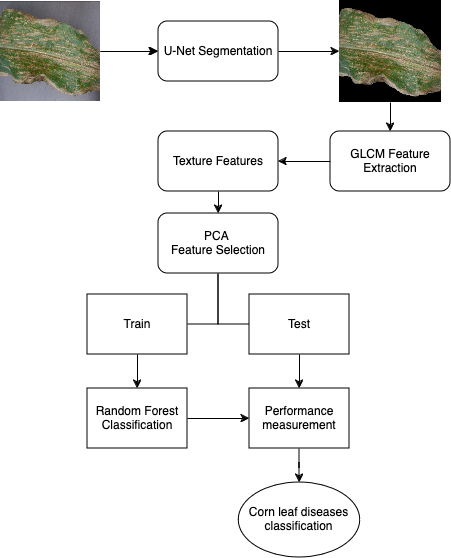
\includegraphics[width=0.95\linewidth]{images/comvis-diagram.drawio(2).png}
    \caption{The flow through the method offered.}
    \label{fig:proposedmethod}
\end{figure}

\subsection{Dataset}

We obtained the dataset for corn diseases from the Plant Village Dataset.  The dataset used in this study is images of diseases on corn leaves. The dataset has four classes, each with 7317 images: Healthy, Common Rust, Northern Leaf Blight, and Gray Leaf Spot (see Fig. \ref{fig:dataset sample}). Divide the dataset into 80\% for training data and 20\% for test data.

\begin{figure}[t]
    \centering
    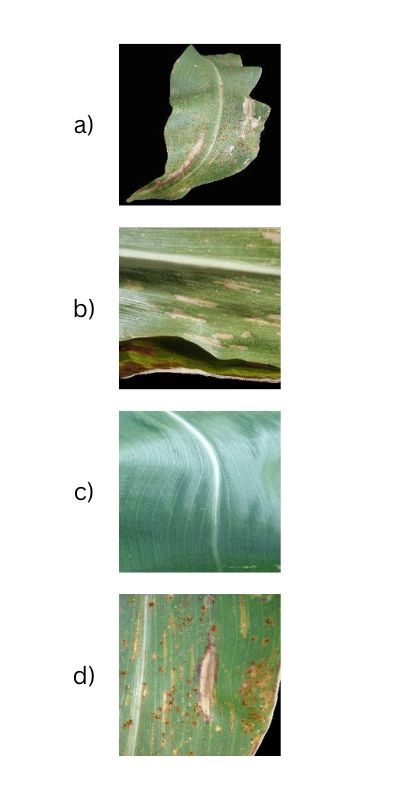
\includegraphics[width=0.4\textwidth]{images/gambar_sample.jpg}
    \caption{a) Common Rust, b) Northern Leaf Blight, c) Healthy Leaf, d) Grey Leaf Spot}
    \label{fig:dataset sample}
\end{figure}

\subsection{Preprocessing}

\subsubsection{Segmentation}

The image is first segmented to extract meaningful information contained in the image. The author wants to highlight the leaf element in the image, which will be the object of classification later. Apply U-Net for segmentation, which has performed well and is widely used \cite{Bhagat2022,Ronneberger2015}. Applying U-Net as the architecture of the segmentation process will provide better results than existing segmentation methods, such as thresholding or edge-based. This segmentation aims to separate the leaf surface from the surroundings. Leaf surface information is the main one to extract and compare information about diseases experienced by corn leaves. U-Net architecture is shown in Fig. \ref{fig:u-net}.

\begin{figure}[h]
    \centering
    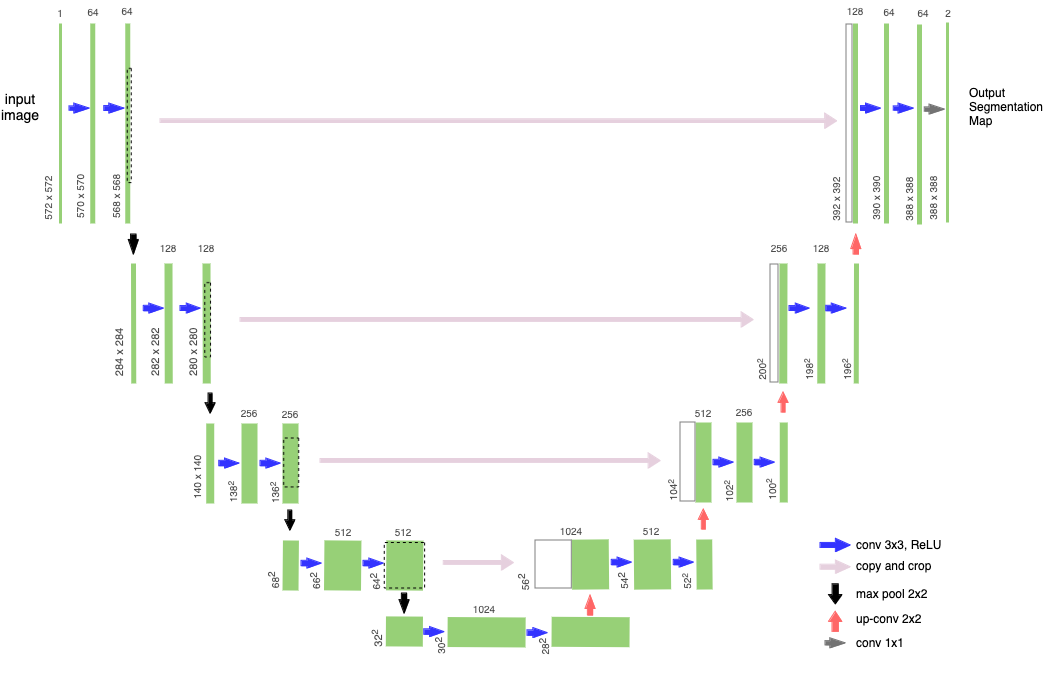
\includegraphics[width=\linewidth]{images/u-net_architecture.drawio.png}
    \caption{A U-Net model for semantic segmentation, featuring a series of convolutional layers with decreasing stride in the encoder, followed by upsampling and concatenation operations in the decoder to refine the segmentation map.}
    \label{fig:u-net}
\end{figure}

\subsubsection{Grayscaling}

The segmented image is still an RGB image. Convert it to grayscale before processing it with the Gray-Level Co-occurrence Matrix. Summing the values of each illuminated pixel converts an image to a grayscale. Apply the grayscale formula as shown in \ref{eq:1}. Lighting and shadow conditions, common in field environments, were addressed using histogram equalization and shadow removal techniques to enhance grayscale image quality. Future improvements in preprocessing could further mitigate these challenges, especially in cases where disease-affected areas are obscured by foliage.

\begin{equation} \label{eq:1}    
Y = 0.299 \cdot R + 0.587 \cdot G + 0.114 \cdot B
\end{equation}

where \( Y \) is the grayscale value, and \( R \), \( G \), and \( B \) are the red, green, and blue components of the pixel, respectively.

\subsection{Feature Extraction using GLCM}

Use the Gray-Level Co-occurrence Matrix technique to extract texture features from images \cite{Utaminingrum2022}. Segment the image again and extract its features. The method applied is a Gray-Level Co-occurrence Matrix (GLCM), which extracts texture features in images using gray-level transitions between 2 neighboring pixels. This technique uses statistical methods to determine the relationship between the values of adjacent pixels in a digital image to extract many features \cite{Utaminingrum2023,Priyanka2020}. 

The steps in GLCM calculation are as follows \cite{Utaminingrum2023}:

\begin{enumerate}
    \item Determine the values of distance ($d$) and angle ($\theta$).
    \item Perform iteration by providing a pair of values of two adjacent pixels based on $d$ value. Fig. 1 shows how the values of the GLCM matrix are obtained.
    \item Sum the GLCM matrix by transposing the GLCM matrix to obtain a symmetric GLCM matrix.
\end{enumerate}

GLCM extracts seven features: Contrast, Dissimilarity, Homogeneity, Energy, ASM, Entropy, and Correlation. Contrast is the difference between colors that makes an object distinguishable. Equation (\ref{eq:2}) is the formula for contrast. After the contrast feature, the next feature extracted is dissimilarity. Dissimilarity measures the dissimilarity of the image texture, as in (\ref{eq:3}). Next, extract the homogeneity feature. Homogeneity measures how closely the distribution of elements in the GLCM approximates its diagonal, as in (\ref{eq:4}). The following extracted features are Energy and Angular Second Moment (ASM). Energy measures the uniformity of an image's texture, while ASM is the root of Energy, as (\ref{eq:5}) and (\ref{eq:6}), respectively. Lastly, examine the correlation features from the GLCM matrix, as shown in (\ref{eq:7}).

This formulation will combine texture features based on the distance and angle used. This research will use 1,2,3,4,5 distances and 0\degree, 45\degree, 90\degree, and 135\degree, respectively. This combination of distances and angles will produce 120 features.

\begin{equation} \label{eq:2}
Contrast=\sum_{i}\sum_{j}(i-j)^2 p(i,j,d,\theta)
\end{equation}

\begin{equation} \label{eq:3}
Dissimilarity=\sum_{i}\sum_{j}p(i,j,d,\theta)|i-j|
\end{equation}


\begin{equation} \label{eq:4}
Homogeneity=\sum_{i}\sum_{j}\frac{p(i,j,d,\theta)}{1+|i+j|}
\end{equation}


\begin{equation} \label{eq:5}
Energy=\sum_{i}\sum_{j}p(i,j,d,\theta)^2
\end{equation}

\begin{equation} \label{eq:6}
ASM=\sqrt{Energy}
\end{equation}


\begin{equation} \label{eq:7}
    Correlation=[\sum\sum((ij)p(i,j,d,\theta)-\mu_x\mu_y)]
\end{equation} 

where, $p$\ is probability. $i$\ is gray level of location pixels (x,y). $j$ is gray level of pixels at distance $d$ and orientation angle $\theta$. $d$ is pixel distance at orientation angle $\theta\degree$. $\theta$ is orientation angle of the main pixel $(0\degree, 45\degree, 90\degree, 145\degree)$. $\mu_x\mu_y$ is average of the probabilities $x$ and $y$.


\subsection{Feature selection using PCA}

This research offers GLCM feature selection using Principal Component Analysis.

Principal Component Analysis (PCA) is a statistical technique for dimensionality reduction, data compression, and feature extraction. It transforms a large set of variables into a smaller one that still contains most of the information in the original set. PCA achieves this by identifying the directions (principal components) along which the variation in the data is maximal.

Calculate the number of variance ratios within the range of components. This calculation helps determine the number of components or features to use. This research will try five feature variables, each with 120, 90, 60, 30, and 10 features. Measure the prediction accuracy using the Random Forest algorithm for each number of features.

\subsection{Classification using Random Forest}

The GLCM feature extraction results were split into 80\% training and 20\% test data. The training and test data are used to train the Random Forest algorithm and map images into four classes. 

Random Forest is an ensemble learning method used for classification, regression, and other tasks that operates by constructing multiple decision trees during training and outputting the class (classification) or mean prediction (regression) of the individual trees \cite{Xu2019}. It is a robust algorithm because it can reduce overfitting by averaging multiple decision trees and providing a robust prediction.

The stages in implementing Random Forest are as follows.
\begin{enumerate}
    \item Data sampling: Create multiple subsets of the original data using bootstrapping (random sampling with replacement).
    \item Building Trees: For each subset, grow a decision tree without pruning.
    \item Feature selection: At each node in a tree, select a random subset of features and determine the best split among them.
    \item Voting: For classification, each tree in the forest votes for a class, and the class with the majority votes is chosen. 
\end{enumerate}

The implementation of Random Forest can be derived from (\ref{eq:8}).
\begin{equation} \label{eq:8}
    \hat{y} = \arg\max_{c \in \mathcal{C}} \sum_{b=1}^B \mathbf{1}\{T_b(\mathbf{x}) = c\}
\end{equation}

where, \( \hat{y} \) is the predicted class. \( \mathcal{C} \) is the set of possible classes. \( B \) is the number of trees in the forest. \( T_b(\mathbf{x}) \) is the prediction of the \( b \)-th tree for the input \( \mathbf{x} \). \( \mathbf{1}\{ \cdot \} \) is the indicator function that returns 1 if the argument is true and 0 otherwise.


\subsection{Model evaluation}

The success rate is necessary to determine how accurate and reliable a model is. This research will measure accuracy, computing time, precision, and recall.

\subsubsection{Accuracy}

The accuracy value shows how successful and accurate the algorithm applied to the test data is. The formula used is (\ref{eq:9}) \cite{Nyasulu2023}:

\begin{equation} \label{eq:9}
    Accuracy=(\frac{TP+TN}{TP+TN+FP+FN})
\end{equation}

where,
\begin{itemize}
    \item TP: True Positive, the number of correct positive predictions.
    \item TN: True Negative, the number of correct negative predictions.
    \item FN: False Negative, the number of false negative predictions.
    \item FP: False Positive, the number of false positive predictions.
\end{itemize}

\subsubsection{Precision}

The precision value measures how accurate the prediction results are from true positives and false positives. The precision formula is in (\ref{eq:10}) \cite{Nyasulu2023}.

\begin{equation} \label{eq:10}
Precision=(\frac{TP}{TP+FP})
\end{equation}

\subsubsection{Recall}

Recall measures how well the application provides prediction results for the number of true positive and false negative data points. Here is the recall in (\ref{eq:11}) \cite{Nyasulu2023}.

\begin{equation} \label{eq:11}
Recall=(\frac{TP}{TP+FN})
\end{equation}

\section{Results and Discussion}

This study aims to analyze the results of corn disease classification without feature selection and the results of selection on GLCM features using PCA. Then, it will determine the best combination based on accuracy, precision, recall, and computing time.

Fig. \ref{fig:segmentation-result} shows the difference in results from segmentation methods with UNet on one sample. The separation between the leaf surface and the background is more visible in UNet compared to the results of other segmentation methods. This segmentation result can facilitate feature extraction by GLCM by only analyzing the leaf surface.

\begin{figure}[t]
  \centering
  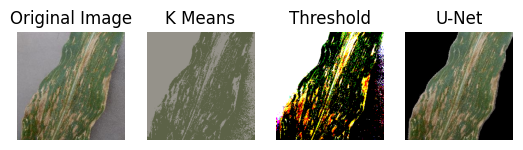
\includegraphics[width=\linewidth]{images/segmentation_result.png}
  \caption{Comparison of segmentation results of K-Means, thresholding, and UNet methods. UNet can undoubtedly separate leaves from their background.}
  \label{fig:segmentation-result}
\end{figure}


Table \ref{table:1} shows the results of prediction measurements on variations in the number of GLCM features. For feature 120, do not apply feature selection using PCA. Based on Table \ref{table:1}, the accuracy is similar for each number of features, namely in the 82\% to 87\% range. Decreasing the dimensionality of the training data from PCA did not contribute to decreasing the prediction accuracy of the model.

The model achieved an accuracy of 0.87, with a precision of 0.87, recall of 0.87, and F1-score of 0.87, across all feature sets. These metrics reflect the balanced performance of the classifier across all evaluated classes.

The similar performance between 10 and 120 features suggests that the most critical information was captured by the top 10 features, while additional features did not significantly improve classification. However, the intermediate feature sets (30-90) may have introduced noise or redundant information, leading to poorer performance. This outcome highlights the importance of selecting only the most informative features for efficient classification.

% The graph \ref{fig:accuracy-results} visualizes the differences in accuracy in more detail for each number of features. Feature 120 (without feature selection) has the same accuracy as feature 10 (with feature selection). Meanwhile, from feature 90 to 30, there is a decrease in accuracy. The result shows a minimum number of GLCM features that are significant in detecting disease on corn leaves with an accuracy level of 87\%. Therefore, applying PCA to reduce the number of features to an exact number will have an accuracy comparable to the overall number of GLCM feature combinations.

The results show that the computing time also decreased as the number of PCA dimensions for GLCM features decreased. Fig. \ref{fig:time-results} illustrates significant differences in the ranges of several features that led to reduced computing time. The number of features impacts the time required to execute the algorithm or classification method. Lower computing time will positively impact algorithm applications for devices with low specifications.

\begin{table}[ht]
    \centering
    \caption{The prediction results are based on the number of PCA dimensionality of GLCM features in the test data.}
    \begin{tabularx}{\linewidth}{|c|c|c|c|c|}
        \hline
        \textbf{Feature Dimensionality} & \textbf{Accuracy} & \textbf{Precision} & \textbf{Recall} & \textbf{F1} \\
        \hline
        120 (No Feature Selection) & 0.87 & 0.87 & 0.87 & 0.87 \\
        90 & 0.84 & 0.83 & 0.84 & 0.84 \\
        60 & 0.83 & 0.83 & 0.83 & 0.83 \\
        30 & 0.82 & 0.82 & 0.82 & 0.82 \\
        10 & 0.87 & 0.86 & 0.87  & 0.87\\
        \hline
    \end{tabularx}
    \label{table:1}
\end{table}

\begin{figure}[h]
    \centering
    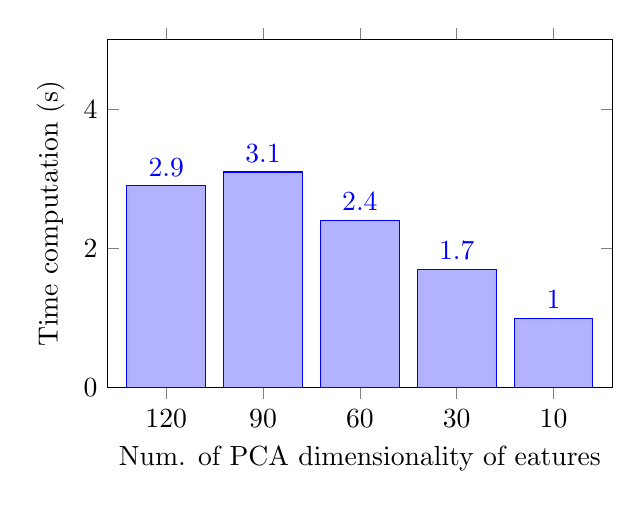
\begin{tikzpicture}
        \begin{axis}[
            ybar,
            symbolic x coords={120, 90, 60, 30, 10},
            xtick=data,
            ymin=0.0,
            ymax=5.0,
            ylabel={Time computation (s)},
            xlabel={Num. of PCA dimensionality of eatures},
            nodes near coords,
            bar width=1cm,
            width=8cm,
            height=6cm,
            enlarge x limits={abs=0.75cm}
        ]
        \addplot coordinates {(120, 2.9) (90, 3.1) (60, 2.4) (30, 1.7) (10, 1.0)};
        \end{axis}
    \end{tikzpicture}
    \caption{Graph of average computation time for each number of PCA dimensionality of GLCM features.}
    \label{fig:time-results}
\end{figure}

\section{Conclusion}

Classifying diseases in corn is crucial for preventing and minimizing economic losses caused by corn diseases. The results of this study demonstrate that the proposed method can quickly classify corn diseases. This method also meets the need for a reliable classification model without requiring extensive computing infrastructure. Testing this method on mobile devices is still necessary to gather more comprehensive data. In real-world applications, the use of IoT devices could be extended beyond mobile phones to include drones or mounted sensors that automate the capture of plant disease images. This method minimizes manual labor and enhances the practicality of using the proposed model in large-scale agricultural settings.

\section{Acknowledgement}

The Faculty of Computer Science has been instrumental in my academic journey. I am deeply grateful for their generous funding that enabled me to join in the international conference. This opportunity allowed me to present my research topic on Corn Leaf Diseases Classification and gain valuable insights from leading researchers in the field.

\bibliographystyle{IEEEtran}
\bibliography{references}

\end{document}
